In most cases, it is necessary to consider a more general transformation than a
simple translation; generally, this transformation will not be linear. In the
case of univariate data, we will have functions
$x_i: \mathcal{T} \rightarrow \mathbb{R}$, in such a way that we can understand
the problem as the search for an appropriate parameterization of our data,
according with the intrinsic structure of the dataset.

We will consider the functions $\gamma_i: \mathcal{T} \rightarrow \mathcal{T}$,
referred to as warping functions in te related literature, that we will use to reparametrize the domain, through which we will be able to
obtain the curves registered by means of composition of functions, i.e.,

\begin{equation}[]{Warping registration}
x_i^*(t)=x_i(\gamma_i(t)) = x_i \circ \gamma _i.
\end{equation}

So that the alignment does not alter the structure of out functional data,
these functions $\gamma_i$ must be boundary-preserving dipheomorphisms. In the
case where the domain of the functions $\mathcal{T}$ is an interval $[a,b]$, the
warpings will be strictly increasing functions that fix the bounds of the
domain, i.e., $\gamma_i(a)=a$ and $\gamma_i(b)=b$, as could be seen in the
figure \ref{FIG:WARPINGS}.

\begin{figure}[Set of warping functions]{FIG:WARPINGS}{Set of warping functions defined in $\mathcal{T}=[0,1]$}
  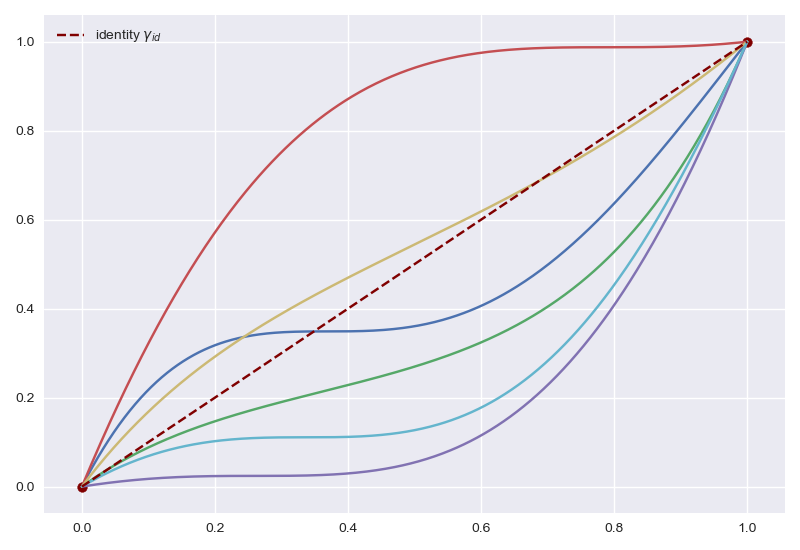
\includegraphics[width=8cm]{random-warpings}
\end{figure}


Without loss of generality, in the following sections, we
will assume that $\mathcal{T}=[0,1]$, because the general case
$\mathcal{T}=[a,b]$ can be reduced to this with an affine transformation. Also,
we will denote the set of these warping functions as $\Gamma$.
